\section{Evaluation}
\label{evaluation}

The following section will provide an evaluation of the two schemes based on an automated benchmark implemented as part of the C++ library described in section \ref{implementation}. The benchmark measures the following metrics of each LSH scheme:

\begin{itemize}
  \item \textbf{Insertion throughput:} How many items can be inserted into the data structure per second on average?
  \item \textbf{Query throughput:} How many queries can be performed against the data structure per second on average?
  \item \textbf{Bucket distribution:} How many buckets are created per partition on average?
  \item \textbf{False negative rate:} How many false negatives occur per query on average?
\end{itemize}

The benchmark performs a 1-NN search in each of three configured tables: A brute force table, a classic table, and a covering table. The purpose of the brute force table is to establish the ground truth by locating the exact nearest neighbour for each of the query items. This ground truth is then used for determining if a false negative has been encountered for each of the query results in the classic and covering tables.

\textbf{Note:} The construction time of the data structure itself under the different schemes is not considered by the benchmark, as we consider this a pre-processing step. However, the construction time required for covering LSH is significantly higher than that required by classic LSH due to the increased complexity of constructing covering families of hash functions. This issue is tackled in \cite{DBLP:journals/corr/PhamP16} which proposes the so-called \textit{fast covering LSH} scheme for efficiently constructing covering families.

\paragraph{Dataset} The dataset used for the evaluation is a pre-processed version of the \texttt{ANN\_SIFT1M} set distributed as part of the Multi Index Hashing (MIH) library located at \url{https://github.com/norouzi/mih}.

This dataset is created specifically for the evaluation of approximate nearest neighbour search algorithms and is a set of 1 million image feature vectors of 128 dimensions, plus an additional 10,000 query vectors. The version distributed alongside the MIH library is however binarised to vectors of 64 dimensions using LSH, which better suits the purpose of our evaluation.

\paragraph{Parameters} Our choice of parameters follows that of the experiments carried out in \cite{DBLP:journals/corr/PhamP16}. That is, for a given radius $r$, we set the number of partitions to use in the classic table to $l = 2^{r + 1} - 1$ and the number of bits to sample to $k = 􏰢\frac{\log(1 - \delta^{\frac{1}{l}})}{\log(1 - \frac{r}{d})}$.􏰣 The benchmark is run for both $\delta = 0.01$ and $\delta = 0.001$. For the covering table we just need the radius $r$.

\subsection{Results}

The results were obtained by running the benchmark on a 2.8 GHz Intel Core i5 processor with a 3 MB L3 cache and 8 GB of DDR3 memory. Due to the limited amount of memory available, we have only been able to provide results for $r \in \{2,\ldots,5\}$.

\subsubsection{Bucket distribution}

We start by considering the average number of buckets created per partition as this turned out to be the defining difference between the two LSH schemes. As can be seen in figure ~\ref{fig:buckets-per-partition}, the average number of buckets per partition is in the case of classic LSH dependent on the radius, and as such the number of bits sampled.

This, however, is not the case in covering LSH where the number of buckets per partition remains constant for every radius. This ties into the way covering LSH correlates the bits to sample from vectors, causing the number of buckets per partition to depend on the input set rather than the radius.

The increased number of buckets does however cause an increase in the total memory usage of the data structure, as each bucket in our implementation has an overhead of 24 bytes on a 64-bit operating system.

\begin{figure}[ht]
  \centering
  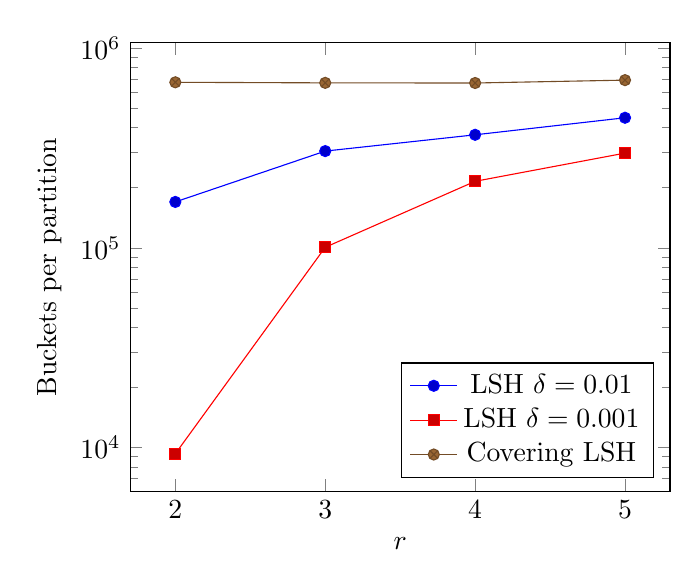
\begin{tikzpicture}
    \begin{semilogyaxis}[
      xlabel = {$r$},
      ylabel = {Buckets per partition},
      xtick = data,
      legend pos = south east
    ]
      \addplot coordinates {
        (2, 169815.43)
        (3, 305179.47)
        (4, 368261.81)
        (5, 448140.33)
      };

      \addplot coordinates {
        (2, 9310.57)
        (3, 100652.33)
        (4, 215357.87)
        (5, 298153.22)
      };

      \addplot coordinates {
        (2, 674554.00)
        (3, 670221.60)
        (4, 669083.68)
        (5, 691636.11)
      };

      \legend{LSH $\delta = 0.01$, LSH $\delta = 0.001$, Covering LSH}
    \end{semilogyaxis}
  \end{tikzpicture}

  \caption{Comparison of bucket distribution}
  \label{fig:buckets-per-partition}
\end{figure}

\subsubsection{Insertion throughput}

As can be seen in figure ~\ref{fig:insertions-per-second}, the insertion throughput of the two LSH schemes follows the same trend as the bucket distribution, albeit in reverse. As such, covering LSH performs worse than classic LSH due to the added overhead of having to construct more buckets. While the difference in bucket distribution is rather significant between the two schemes, the difference in insertion time is negligible in comparison.

\begin{figure}[ht]
  \centering
  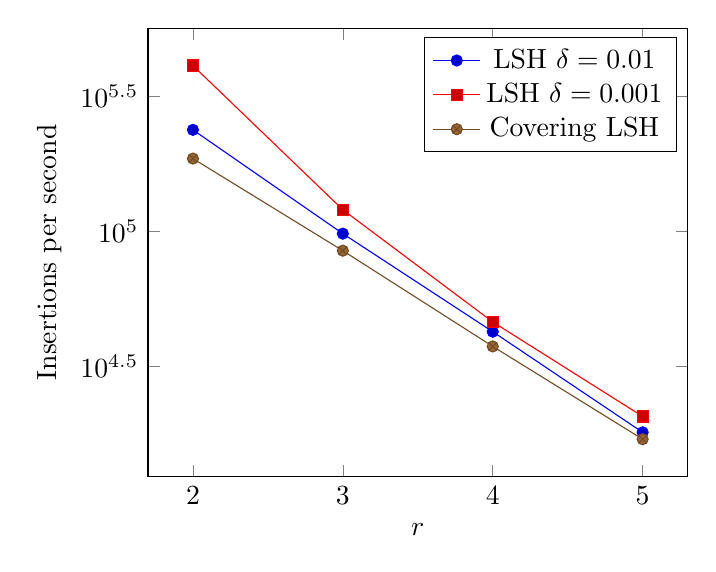
\begin{tikzpicture}
    \begin{semilogyaxis}[
      xlabel = {$r$},
      ylabel = {Insertions per second},
      xtick = data
    ]
      \addplot coordinates {
        (2, 237736.94)
        (3, 98187.51)
        (4, 42593.97)
        (5, 18074.10)
      };

      \addplot coordinates {
        (2, 411106.15)
        (3, 120359.67)
        (4, 46280.57)
        (5, 20693.81)
      };

      \addplot coordinates {
        (2, 186131.05)
        (3, 84934.71)
        (4, 37573.59)
        (5, 17047.07)
      };

      \legend{LSH $\delta = 0.01$, LSH $\delta = 0.001$, Covering LSH}
    \end{semilogyaxis}
  \end{tikzpicture}

  \caption{Comparison of insertion throughput}
  \label{fig:insertions-per-second}
\end{figure}

\subsubsection{Query throughput}

Our initial expectations of the query throughput of the covering LSH scheme was that it would follow the same trend as the insertion throughput, i.e. be slightly less performant than the query throughput of classic LSH. As seen in figure ~\ref{fig:queries-per-second}, this is however far from the case. Due to the bucket distribution of covering LSH, we can can assume that it is able to produce candidate sets that on average are smaller than those produced by classic LSH. The improved filtering efficiency in turn has a significant effect on the query throughput, making covering LSH perform much better than classic LSH on the evaluated dataset.

\begin{figure}[ht]
  \centering
  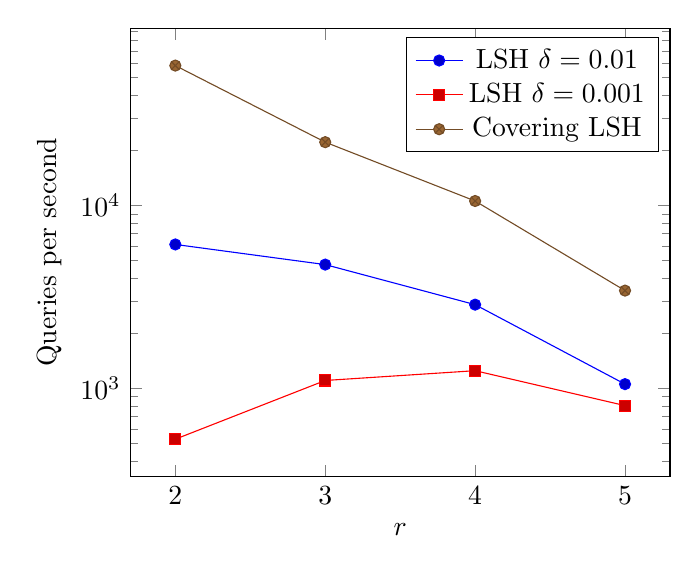
\begin{tikzpicture}
    \begin{semilogyaxis}[
      xlabel = {$r$},
      ylabel = {Queries per second},
      xtick = data
    ]
      \addplot coordinates {
        (2, 6118.88)
        (3, 4747.76)
        (4, 2866.80)
        (5, 1053.48)
      };

      \addplot coordinates {
        (2, 526.67)
        (3, 1103.17)
        (4, 1247.75)
        (5, 803.80)
      };

      \addplot coordinates {
        (2, 58216.55)
        (3, 22187.94)
        (4, 10574.71)
        (5, 3421.63)
      };

      \legend{LSH $\delta = 0.01$, LSH $\delta = 0.001$, Covering LSH}
    \end{semilogyaxis}
  \end{tikzpicture}

  \caption{Comparison of query throughput}
  \label{fig:queries-per-second}
\end{figure}

\subsubsection{False negative rates}

The last metric considered, and likely the most important one, is the false negative rates of the two LSH schemes. As can be seen in figure ~\ref{fig:false-negatives-per-query}, the number of false negatives per query is exactly as one would expect; classic LSH produces false negatives proportional to $\delta$ and covering LSH produces no false negatives at all as is also shown in the experiments conducted in \cite{DBLP:journals/corr/PhamP16}.

\begin{figure}[ht]
  \centering
  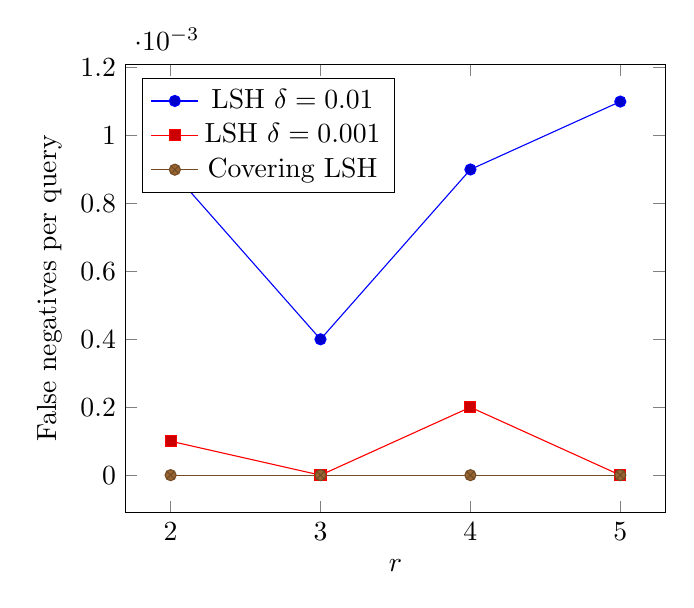
\begin{tikzpicture}
    \begin{axis}[
      xlabel = {$r$},
      ylabel = {False negatives per query},
      xtick = data,
      legend pos = north west
    ]
      \addplot coordinates {
        (2, 0.0009)
        (3, 0.0004)
        (4, 0.0009)
        (5, 0.0011)
      };

      \addplot coordinates {
        (2, 0.0001)
        (3, 0.0000)
        (4, 0.0002)
        (5, 0.0000)
      };

      \addplot coordinates {
        (2, 0.0000)
        (3, 0.0000)
        (4, 0.0000)
        (5, 0.0000)
      };

      \legend{LSH $\delta = 0.01$, LSH $\delta = 0.001$, Covering LSH}
    \end{axis}
  \end{tikzpicture}

  \caption{Comparison of false negative rates}
  \label{fig:false-negatives-per-query}
\end{figure}
